\documentclass[sigconf,authorversion,nonacm]{acmart}
\bibliographystyle{ACM-Reference-Format}
\usepackage{hyperref}
\usepackage{alltt}

%TODO: disable folios
\settopmatter{printfolios=true}

\definecolor{ForestGreen}{RGB}{34,139,34}

%\widowpenalties 4 0 9000 10000 10000

%%%%%Prof Zhou's Rant on Citations, Punctuation, and Quotes %%%%%%
%%%
%%% Yes - ...of seventy-two''~\cite{42}.
%%% Yes - ...of seventy-two.''\footnote{42}
%%%
%%% NO! - ...of seventy-two.''~\cite{42}.
%%%
%%% https://advice.writing.utoronto.ca/wp-content/uploads/sites/2/quotations.pdf
%%%
%%%%%%%%%%%%%%%%%%%%%%%%%%%%%%%%%%%%%%%%%%%%%%%%%%%%%%%%%%%%%%%%%%

% 8-10 pagecount.

\begin{document}
\title[Visualizing CAD changes with Boolean Differences]
{Visualizing CAD changes with Boolean Differences\\
	\normalsize{Group 25 Final Report}}
%I'd like to remove the 'group 25 report' from the title, not really sure where to put it though .

\author{Amos Hebb}
\affiliation{\institution{University of Toronto}}
\email{a.hebb@mail.utoronto.ca}
\author{Yilong Wang}
\affiliation{\institution{University of Toronto}}
\email{yilongece.wang@mail.utoronto.ca}
\author{Zhenyue Yu}
\affiliation{\institution{University of Toronto}}
\email{zhenyue.yu@mail.utoronto.ca}

\makeatletter
\def\@ACM@checkaffil{% Only warnings <<<<<<<<<<<<<<<<
	\if@ACM@instpresent\else
		\ClassWarningNoLine{\@classname}{No institution present for an affiliation}%
	\fi
	\if@ACM@citypresent\else
		\ClassWarningNoLine{\@classname}{No city present for an affiliation}%
	\fi
	\if@ACM@countrypresent\else
		\ClassWarningNoLine{\@classname}{No country present for an affiliation}%
	\fi
}
\makeatother

\maketitle

\section{Introduction}

In today's fast-paced and complex digital world, Computer-Aided Design (CAD) has become an indispensable tool in various industries, including engineering, architecture, and manufacturing.
However, with the increasing use of distributed CAD practices, new challenges have emerged in tracking changes made to CAD files.
To address this issue, our report explores the challenges associated with distributed Computer-Aided Design (CAD) practice and investigates whether visualizations of Boolean differences can summarize changes between CAD file versions.
Our report proposes two experiments to test the effectiveness of Boolean differences in summarizing changes. The first experiment involves timed cherry-picking tasks where participants are divided into two groups, one with access to Boolean differences between CAD file versions and the other without.
The second experiment involves summarization tasks where participants are again divided into two groups, one with access to Boolean differences and the other without.
Our report highlights the importance of this research in providing a faster and more accurate alternative to the current methods used to capture CAD file changes, as well as contributing to the development of techniques and tools for visualizing differences between complex files. Our report also acknowledges the challenges associated with the lack of standardization and the difficulty in interpreting visual differences from Boolean differences for some types of changes.
Finally, our report predicts that Boolean differences will facilitate the reversing process significantly in the cherry-picking experiment and help users better summarize changes in the summarization experiment.

\subsection{Motivation}
Computer-Aided Design (CAD) collaboration has been studied since the early days of CAD research, but standardized metrics and experimental procedures for synchronous, collaborative CAD research are lacking in the literature. In order to keep up with the increasingly rapid pace of innovation and consumer demand for customization, businesses must engage in global design chains and work collaboratively with partners both locally and overseas.
This type of collaboration allows companies to gain a competitive edge by leveraging the strengths and expertise of different team members and partners in diverse locations.
As the world becomes more interconnected, the ability to collaborate effectively across distances and cultural barriers becomes increasingly important for companies seeking to succeed in today's fast-paced marketplace~\cite{fuh2005advances}.
In modern product design, manufacturing, and analysis, there is a growing need for collaboration in distributed environments. This collaboration is essential both technically and commercially, and it is critical to develop new collaborative design tools or update traditional standalone CAD systems to become collaboration native.
With the increasing complexity of products, it is necessary to involve a team of experts with different specializations, and collaboration tools can facilitate communication, increase productivity, and reduce errors~\cite{fuh2005advances}.

Additionally, as the Covid-19 pandemic spread rapidly across the globe in 2020 and 2021, CAD design collaboration became more important than ever in the industry.
With team members working from various locations, the process of checking CAD designs in and out of production data management systems has become more complex.
This has further amplified the typical issues that arise with production data management, such as version control and collaboration, making it even more critical to develop effective strategies for managing CAD files remotely.
As a result, there is a growing need for innovative solutions that can help teams efficiently manage their design files and collaborate effectively, regardless of their location~\cite{armstrong}.
Our motivating paper is from Cheng et al.~\cite{cheng2023age} which identifies challenges associated with distributed Computer-Aided Design (CAD) practice. One of the challenges is a lack of change summarization support between file versions.
Teams currently rely on their memory or tedious Excel spreadsheets to capture changes between different versions of CAD files, which is time-consuming and prone to errors. Collaborating on CAD design is essential to effective product development.
Facilitating the team to work together increases checkpoints, provides unbiased feedback and reviews, and adds complementary expertise to optimize the final production part.
\subsection{Research Question}
In this report, we present a mixed method to answer exploratory research questions (RQ) about collaborative CAD.
We have a particular interest in determining whether visual representations of Boolean differences can effectively summarize the modifications between various versions of a CAD file.
To figure this out, we study the following questions:

\textbf{RQ1: Does Boolean difference visualization help people understand the variations between different versions of CAD files?}

\textbf{RQ2: Does Boolean difference visualization impact people's ability to interpret and summarize changes between different CAD files?}

The main objective of this research is to evaluate whether Boolean differences can effectively summarize changes between Computer-Aided Design (CAD) file versions.
Boolean differences are a visualization technique inspired by git diff and 3D art workflows that can be applied to 3D solids to create new solids.
By investigating whether these new solids can help designers understand changes between versions of CAD files, this research aims to provide a faster and more accurate alternative to the current methods used to capture CAD file changes.
Moreover, this study aims to contribute to the development of techniques and tools for visualizing differences between complex files, which can have implications for other domains where changes in complex files should be summarized.
The importance of this research lies in the fact that it can help CAD users identify and track changes between versions of files more efficiently.
This, in turn, can lead to faster and more accurate design iterations, ultimately resulting in better-designed products.
Additionally, this research can help advance the field of visualization by developing new techniques and tools for visualizing differences between complex files.
Such tools can be useful in various domains, including engineering, architecture, and graphic design.
\subsection{CAD}

CAD or computer-aided design refers to the use of computer software to create, modify, and optimize design processes.
It has revolutionized the way engineers and designers work by simplifying the design process and increasing the accuracy and precision of designs.
CAD software can create both 2D drawings and 3D models, enabling designers to create complex designs with ease. The use of CAD can help streamline the designer's workflow, leading to increased productivity and faster turnaround times.
Additionally, CAD can improve the quality and level of detail in the design, making it easier to communicate with stakeholders, clients, and manufacturers.
It can also contribute to a manufacturing design database, allowing for the creation of future designs that can be built upon existing ones.
CAD software is utilized to create electronic files that are then utilized for various manufacturing procedures.
CAD is typically utilized together with digital production techniques. CAD/CAM software is utilized to develop items such as electronic circuit boards for use in computers and other devices.
These software tools allow for more precise designs, faster manufacturing processes, and increased efficiency in the production of products.
By streamlining the design and manufacturing process, CAD software has become an essential tool for many industries, including architecture, engineering, and product design~\cite{chai_2020}.

\subsection{OpenSCAD}
OpenSCAD is a software program for solid modeling that is script-based, free, and open-source.
With OpenSCAD, 3D digital designs can be created easily and quickly by manipulating parametric variables that automatically adjust the entire part.
This feature of OpenSCAD enables even those without extensive knowledge in 3D modeling to make simple modifications to existing designs.
By using OpenSCAD, designers can save time and effort while producing accurate and detailed 3D designs~\cite{pearce2015applications}.
The OpenSCAD program is used to create 3D models by defining geometric primitives and then modifying and combining them according to user-defined parameters.
In this project, we chose to use OpenSCAD to create STL files for our dataset. By using OpenSCAD in this way, we were able to accurately compare the performance of different 3D printing methods and evaluate the effectiveness of their proposed techniques.
\subsection{\texttt{.stl} files}

The \texttt{.stl} file format is a representation of the surface geometry of a three-dimensional object common in both CAD and 3D art.
These files are among the \textit{dumb solid} types described in~\cite{cheng2023age}, a neutral file format interoperable between most CAD and 3D art platforms, but missing critical information for CAD practitioners.
\texttt{.stl} files have no way to represent curves, holes, orientation, or distinguish multiple parts in an assembly.
Providing measurements is optional in \texttt{.stl} files. CAD programs usually store this optional information about units.
We hope this tool can be used with any CAD software.
Most CAD programs support exporting models to \texttt{.stl} files and our visualization only relies on surface geometry, making \texttt{.stl} files appealing for producing quick summaries.

\subsection{Git}

Git is a version control system designed by the Linux kernel team to support many coders making changes to text files in a distributed and collaborative way.
Git has become one of the most widely used version control systems and is particularly popular in open-source development projects which face similar challenges to the Linux kernel team.
It has many powerful utilities for manipulating text files.
While Git can handle binary files, the utilities that make it so useful for the collaborative editing of text files do not exist for the complex binary files used in 3D CAD.

\texttt{git diff} is a utility that allows a user to see changes.
These changes are represented by insertions and deletions.
For example, running \texttt{git diff} on a branch where a punctuation mark is added to a hello world program will show unchanged lines in black, insertions in green, and deletions in red.

\begin{alltt}
	fn main ()\{
	\textcolor{red}{   - println!("Hello World");}
	\textcolor{ForestGreen}{   + println!("Hello World!");}
	\}
\end{alltt}

Integrated development environments, git hosts, and other command line tools present git diff with different formatting, layout, and truncation of unchanged code.
There is one thing that unifies every visualization of \texttt{git diff}, the red deletions and green insertions visual.
This red and green visual is ubiquitous in code tools, it is the default presentation of a branch, merge, history, and pull request on every major git platform and every integrated development environment with git support.
These clear visual representations of the differences between different versions of a file make it easy for developers to see what has changed and where.

\texttt{git cherry-pick} is a less common git command.
A developer checks out a target branch and then runs the \texttt{git cherry-pick} with a commit hash to apply a specific commit to the target branch.

It is typically used when there are changes in a \emph{feature} branch that one wishes to apply to the \emph{target} branch.
Instead of merging the entire \emph{feature} branch into \emph{target}, which would bring in all the changes in \emph{feature}, \texttt{git cherry-pick} is used to apply only the specific commits desired.
To do this, a developer would first identify the commits in the \emph{feature} branch that apply the changes they wish to apply.
The developer would \texttt{git checkout} the \emph{target} branch.
The developer then uses \texttt{git cherry-pick} command to apply those commits to the \emph{target} branch.
This creates a new commit in \emph{target} that contains only the changes from the selected commit in \emph{feature}.

A concrete example grounded in 3D CAD.
A company produces a teapot which is modelled in 3D CAD file saved as `main'.
Three changes are made to this initial file.
First, the spout is shortened.
Second, the handle is made square.
Third, the knob on top is made bigger.
The resulting prototype file is saved as `v2', and has a short spout, square handle, and large knob.
After prototyping, the company wishes to keep the short spout and large knob but keep the original handle.
Only the two desired changes from `v2' are applied to `main', resulting in `main2' with the desired changes.

\subsection{Boolean Differences}

The use of Boolean operations, such as intersection, union, and difference, is vital in CAD/CAM systems.
They help create complex geometric structures from simple building blocks, analyze spatial phenomena like interference, and model manufacturing processes such as machining.
In order for these operations to be applied effectively in a CAD/CAM system, algorithms must be able to produce representations of geometric entities that are also closed under these operations.
This ensures that the output from applying Boolean operations can also be used as input for subsequent operations.
Therefore, it is crucial that the domain of a CAD/CAM system be algebraically closed under these operations~\cite{tilove1980closure}.


\section{Literature Review}

The motivating paper for this project is~\citet{cheng2023age}.
We focus specifically on the sections about tooling for version control.
This also identified some existing tools, such as \texttt{onshape.com}, and \texttt{github.com}'s now deprecated \texttt{.stl} diff visualization, both of which attempt to summarize changes with similar visualizations.
We have reviewed this work and evaluated these tools ourselves.

\subsection{Computer-Aided Design Ecosystem is Behind}

This paper by~\citet{cheng2023age} aims to close the academic-practitioner knowledge gap on the state of collaboration with CAD workflows.
After interviews focusing on mechanical CAD, 14 challenges are identified.
It paints a fairly linear history of CAD, first standalone, then distributed, and now collaborative tools have early adopters.
It classifies these with place and time, implying that different-place and same-time collaborative tools are the future.
Our group focuses on improving the different-place and different-time editing, informed by the history of collaboration in code tools.
Distributed code editor, standalone editors combined with a data management system like distributed CAD, have become the norm in programming.
Tools like Git are far newer than synchronous multi-user text editors.
The Mother of All Demos featured a collaborative real-time editor in 1968.~\cite{motherofalldemos}
Many other real-time editors, both 3rd party and included in operating systems, have been created over the last 50 years.
Despite this, different-place, different-time collaboration tools remain far more popular in software development.
We work on improving distributed CAD on the assumption that distributed CAD tools will be popular with CAD practitioners for the same reasons they are popular among software developers.

Some of the specific challenges we hope to address with this work are:

Challenge 1, identified both in literature and interviews was inconsistency in design practices between designers.
Nearly all respondents felt that standards were not enforced.
The only respondent who felt this was not an issue is a CEO asserting that he had resolved this issue using onboarding documents.
Our discussion section contains our thoughts on how a lack of standards may threaten the usefulness of our proposed solution.

Challenge 4, Lack of awareness of collaborators' changes.
We hope that by being able to quickly produce diff views, much like in code, when somebody wishes to understand changes made they can quickly analyze these and understand changes made.

Challenge 8, Lack of interoperability is identified as an issue, something we hope to avoid this issue by proposing a solution relying only on \emph{dumb solids}.

\textbf{Challenge 9, Lack of change summarization support between file versions.}
This is the primary motivating challenge for our project.
Currently, the state of summarization seems to be primarily nothing, with a select few shops using infrequent, stale, or tedious text-based summaries stored in \texttt{.xlsx} files.
We hope that by proposing a visualization that can quickly produce summaries at no cost to the existing workflow, boolean difference visualizations may be adopted to help summarize changes.

\subsection{Evaluating \texttt{onshape.com}}

An existing tool, \texttt{onshape.com}, was evaluated as part of this review.
We were able to create an account and get access to Daniel Riley's Sailboat
%https://cad.onshape.com/documents/a8a8056c3b88f0daf9611dcb/w/221f8e757824bdfe5ba7440b/e/ee5cdb3266c7d6966d32f749
which is a public model which shows a rich combination of \texttt{onshape.com}'s capabilities, in particular, once signed in, the `Versions and History' tab.
This shows a branching visual, with symbols for versions, releases, and the current workspace.
This is initially collapsed, with only versions showing, but expanding a version shows each of the modifications applied.
These modifications are clearly automatically generated, as they are far more granular than would typically be checked into version control manually.
For example, many trivial `Hide', `Show', and long chains of `Drag, Drag, Drag, Drag' and `Move, Move, Move, Move' where the CAD designer seems to be making minor intermediate adjustments.
By default, no `diff' like view is shown.
Instead, the entire document re-loads when clicking on any change.
Right-clicking does reveal a `Compare' option, instead of just `View'.
Many changes throw an error, for example, comparing Main `Show:Keel Mold - Daniel Riley - 1:01 PM Mar 8 2023' to one change before it, the `Move:Rollback bar - Daniel Riley - 12:18 PM Mar 8 2023' removes the render from the screen and shows the error message ``NOT COMPARABLE: Comparing Assemblies is not yet supported.''
Selecting individual components reveals \texttt{onshape.com}'s comparison interface.
The assembly is scattered into an unwieldy exploded view where parts overlap.
Instead of rendering boolean differences, \texttt{onshape.com} renders a before and after visual, and allows a user to scroll a slider left to right while moving the entire exploded state around.
Subtractions are highlighted in red, while new volumes are rendered in blue.
Figure \ref{fig:onshapescreenshot} shows a screenshot with the slider roughly 2/3 toward the new component, showing a partially transparent blue volume, and orange-red holes being cut.

\begin{figure}[t]
	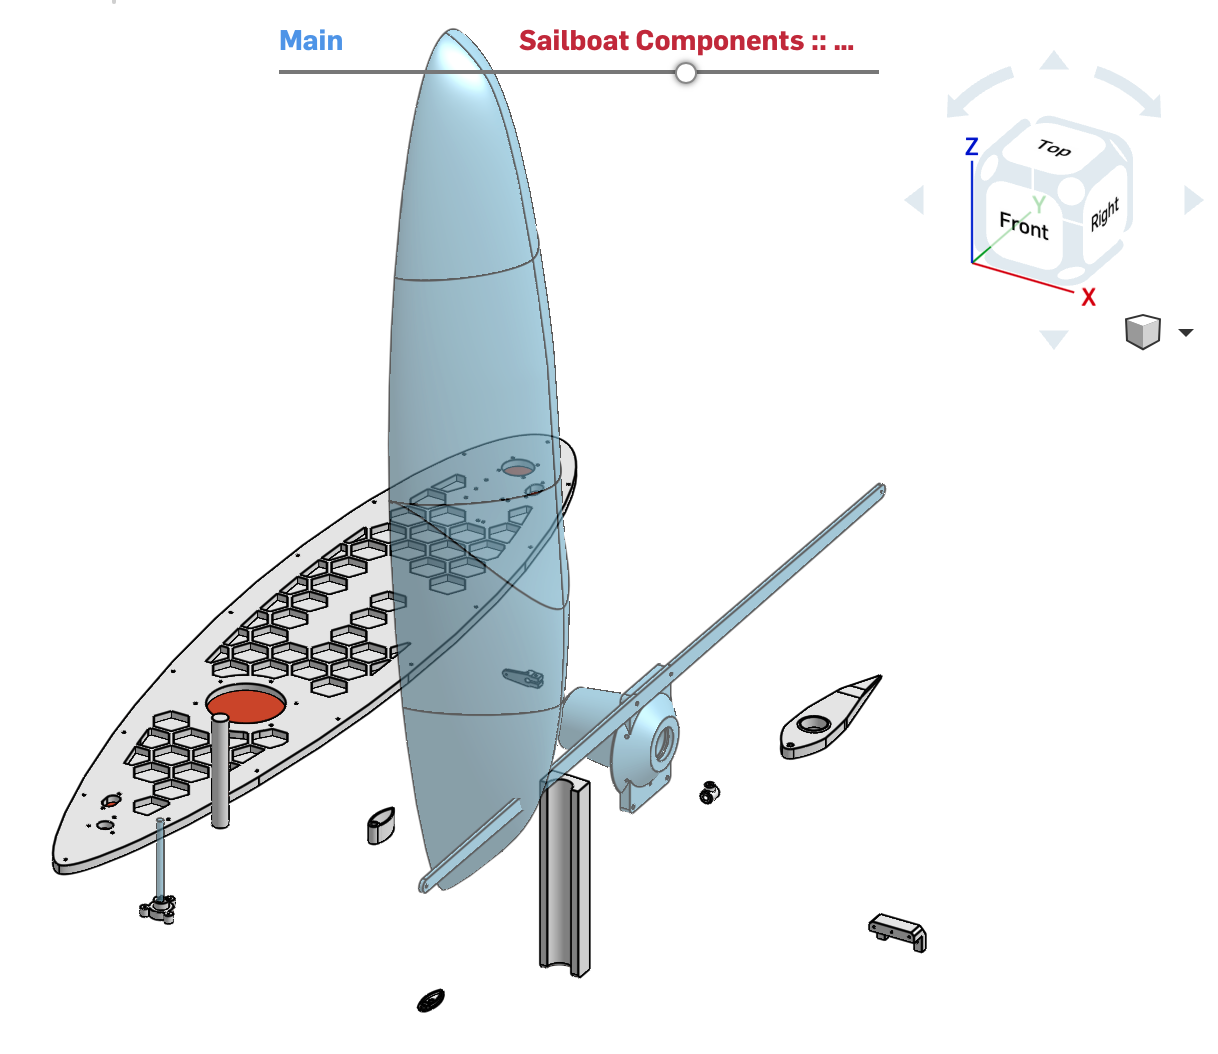
\includegraphics[width=\linewidth]{onshapescreenshot.png}
	\caption{Example of \texttt{onshape.com} compare visual}
	\label{fig:onshapescreenshot}
\end{figure}

\subsection{3D File Diffs on \texttt{github.com}}

As part of a grey literature review, we came across \texttt{github.com}'s 2013 blog post about adding a 3D File Diff view to \texttt{github.com}.~\cite{github_blog_2013}
The blog post presents two visualizations, one uses what the blog refers to as \emph{binary space partitioning}, which is a technique used by 3D video games and is essentially a polygon-based boolean difference.
The second is a slider-based transparency approach which is a rudimentary version of to \texttt{onshape.com}'s compare visualization.

The blog explains how it works.
The visualization is done using \texttt{csgtool} and a Ruby \texttt{csg} gem which appears to have already been in use in 2013 for the git 3D file interface.
\texttt{csgtool} and the ruby gem appear to have been abandoned around 2014, receiving only minor updates bumping dependency versions or correcting typos since.

As of early 2023, there is no 3D File Diff view on \texttt{github.com}.
The specifics of the tool are part of the opaque and closed source code of \texttt{github.com}.
It is not obvious when support stopped.
The comment chain on the file included in the blog post~\cite{death_of_a_diffsman} documents the atrophy of an abandoned project.
The comments reveal a 2013 positive initial reception, a 2017 question about the source code, a 2019 plea to \texttt{github.com} to open source the visualization.
A 2021 post is a disguised advertisement for \citet{3drepoblog}.
This is a BIM tool we did not evaluate, but the founder of this company has published a paper about 3D Diff.~\cite{Dobos}
By 2022, users report this is not working on Firefox or Chrome.

\subsection{3D File Diffs on \texttt{gitlab.com}}

Discouraged that this utility has been abandoned, we took our search to \texttt{gitlab.com}.
The key difference between \texttt{gitlab.com} and \texttt{github.com} is that \texttt{gitlab.com} is open source.
We had hoped that \texttt{gitlab.com} may have copied this feature, but done so in a repo where we could access their implementation.
Inspecting \texttt{gitlab.com} source code quickly reveals a \texttt{.stl} file viewer in the source code.~\cite{gitlabsource}
All 3 files implementing \texttt{.stl} viewing are fewer than 200 lines of generously spaced JavaScript, none of which attempt to compare files.
Due to how concise and readable the code implementing the \texttt{.stl} viewer is, we have decided to explore using the \texttt{threejs.org} webGL library for our interface.

\subsection{3D Diff}

In \citet{Dobos}, previous work recording and replaying actions made in an editor is first summarized.
It mentions 3D Sys's 3D-Diff, a Visual Basic add-on to Catia, which highlights structural differences in CAD models.
This paper focuses on merging tools more than the actuall presentation of the diff.
They perform 2-way and 3-way differencing and merging, compare them, identify differences, and then identify various categories of changes.
Our work only considers the 2-way merge case, where the state can only be one of `Unmodified',`Added', or `Deleted'.
The 3-way case considers multiple different types of deletions and modifications, and well as conflicts.
The visualizations in this work are busy, described as `Overlay' and `Smart', without describing what these visuals represent.
The `Smart' visualization describes using a common ancestor to resolve ambiguities.
It does not appear that this tool is intended for quick summaries of small parts, but instead for comparing large assemblies with major changes.

\section{Methodology}

In this section, we outline the methodology for both the quantitative timed cherry-picking experiment and the qualitative summarization experiment.

\subsection{Timed Cherry-Picking Experiment}

The timed cherry-picking experiment intends to use the accuracy and time that it takes for users to perform a task which requires understanding changes in 3D files as a measurable proxy for `useful summarization'.

\subsubsection{Participants}

The participants are randomly assigned to one of two groups: the experimental group and the control group.
We expect that individual participants may have different levels of experience with each of CAD tools, version control tools, and 3D Art tools.
Recruiting participants with experience in all three will be difficult, so instead we will design our experiment assuming no prior knowledge of any of the above.
We rely on simple random assignment to keep familiarity with the above tools similar between the two groups.
Participants will be informed of the purpose of the experiment and their rights as participants.
Participants who wish to complete this experiment virtually will require a connection to the internet and a web browser with WebGL support.
Participants may also complete this experiment in person using a computer provided by experimenters.
Only completion times and accuracy scores will be recorded with no way to link times back to individual participants.
Participants will be informed that data will be openly available in a public repository that does not issue DOIs.
Participants may withdraw from the experiment at any time and incomplete results will be discarded.

\subsubsection{Task}

The participants will be tasked with reversing a certain part of an object back to a previous version while keeping the rest of the object the same as the final version.

As we assume participants are not familiar with version control, CAD, or 3D art tools, we will not use any existing tools in the experiment to reduce the effect of prior exposure to any of these tools.
Version control tools have specific commands that are not intuitive, and both CAD and 3D art tools have very complex interfaces that could distract participants.
We instead produce a stripped-down interface which only allows participants to view files, and mark files to be included or excluded.

%Attached are screenshots from both the control and experimental group. 
%Figure \ref{fig:controlscreenshot} shows a screenshot of the interface that will be shown to the control group.
The interface has two frames which will render a webGL view \texttt{.stl} renderings of our revisions.
Participants do not need to know file formats, and instead will just refer to changes as an enumerated list of `Original, Change 1, Change 2, Change 3 refer to changes as an enumerated list `Original, Change 1, Change 2, etc.'.
Below each of these frames is a drop-down menu allowing participants to select any of the change files.
The task goal is displayed below these frames.
Below the task goal is a list of changes, along with a radio button group with labels `Include' and `Exclude', which by default will not be selected.
To complete a task, participants must select one of `Include' or `Exclude' for every change, and then press the `Submit' button.
%Figure \ref{fig:experimentscreenshot} shows a screenshot of the interface that will be shown to the experiment group.
The \textbf{experimental group} will have a 3rd frame.
This 3rd frame will render the red and green \emph{diff} view produced by performing boolean operations on the two selected files.


\subsubsection{Procedure}

Before the experiment begins, participants may complete a practice task with assistance from the experimenters as many times as they desire.
Once participants have indicated that they understand the task, experimenters will leave participants to complete the experiment on their own.

Only a `Begin' button will be shown.
Once clicked, a timestamp is logged, and the first task will be presented to the participant.
Once a participant has selected either `Include' or `Exclude' for each of the changes, the `Submit' button will be enabled.
Once a participant clicks the `Submit' button, a second timestamp is logged, along with the `Include' or `Exclude' status of every change.
The task is now over, and the `Begin' button will be shown for the next task.
Once a participant has completed 5 tasks, a `Thanks for participating' screen will be shown.

\subsubsection{Evaluation}

Accuracy will be measured by counting the number of correctly marked changes a participant has submitted to a reference solution.
Every task will have a canonical solution, with a certain set of commits labeled as either `include' or `exclude'.
We will compare this canonical solution to the solution produced by each participant and count the number of correctly labeled changes.
The fraction of correct labels will be our accuracy count, meaning that accuracy will be from 0-1 where 1 is perfect.

Time will be measured in seconds from when participants click the begin button until when they click the submit button.

\subsubsection{Data Analysis}

The first step in analyzing the data is to collect descriptive statistics for both accuracy and time.
These descriptive statistics will be used to confirm our assumptions about the distributions of both of these data.
We will also clean these data to remove any faulty submissions (time is impossibly fast, marked all files `Include', etc.).
Removed rows will be marked `True' in the column \texttt{removed\_from\_analysis} for the public dataset.

We expect times to be normally distributed about the task mean time for each task.
A T-Test will reveal if there is a difference in completion time for the same task between the two groups.
This test will allow us to accept or reject the following hypotheses.

$H_{0}$: Access to the boolean difference view has no impact on the completion time of cherry-picking changes in 3D files.

$H_{Time}$: Access to the boolean difference view reduces mean completion time of cherry-picking changes in 3D files.

As the tasks are fairly obvious, we expect accuracy will follow some long tail distribution with most participants making no mistakes, some making one or two, and rare unusually poor performing participants making many.
Applying statistics that are based on variance and standard deviation to accuracy scores will be impacted by single large outliers.
Instead, we will fit a Poisson distribution to the accuracy scores of each group treating each mistake as a discrete event, and then compare the rate at which mistakes are made between the two groups.
A C-Test~\cite{przyborowski1940homogeneity} is well suited for 0 included Poisson distributions to see if the rate of errors has been changed by the introduction of the Boolean difference view.
This test will allow us to accept or reject the following hypotheses.

$H_{0}$: Access to the boolean difference view has no impact on the accuracy of cherry-picking changes in 3D files.

$H_{Accuracy}$: Access to the boolean difference view reduces the rate of mistakes when cherry-picking changes in 3D files.

A reduction in time and mistakes will indicate that the boolean difference view helps summarize differences, as participants were able to more quickly and more accurately understand changes that had been made in 3D files when they had access to these visualizations.

\subsection{Summarization Experiment}
\subsubsection{Participants and Recruitment}
For the summarization experiment, we plan to recruit participants using purposive sampling. Our target population will consist of individuals with experience in CAD design, as indicated by the inclusion of ``CAD,'' ``CAD Design,''
or similar tags in the Skills section of their LinkedIn profiles. Potential participants will be contacted through LinkedIn messages.

In our initial communication, we will provide an overview of the experiment's purpose and outline the main experimental procedures.
This will help ensure that prospective participants have a clear understanding of what is involved before deciding to participate. As an incentive for their time and effort, those who complete the experiment will receive a \$25 gift card as compensation.

A table will be presented to summarize the demographic information of the participants, including their years of experience with CAD and related information such as whether they use CAD in their daily work.

\subsubsection{Experimental and Control Groups}

The study will use a randomized controlled design, in which participants will be assigned to either the experimental or control group by random assignment. This approach aims to eliminate confounding factors such as prior experience with 3D CAD Design or Git Diff. Assigning participants based on their experience level may introduce systematic error and relying on self-reported experience may not ensure a fair assignment. Therefore, the groups will be assigned by total random assignment.

Both groups will have access to the visualization of 3D objects. The experimental group will also have access to the visualization of Boolean differences. This approach will allow for a comparison between the two groups in terms of their ability to work with the Boolean difference visualization.
\subsubsection{Procedure}
This summarization experiment employs semi-structured interviews to explore the impact of Boolean difference visualizations on participants' ability to identify and describe changes between two 3D CAD objects.
The experiment consists of three distinct stages: preparation, inspection, and summarization, each designed to ensure a smooth and effective process. We anticipate the whole experiment will take 60 to 90 minutes to complete.

During the preparation stage, researchers take care to address participants' rights and confidentiality. They emphasize the voluntary nature of participation and confirm that participants understand the experiment's purpose and methodology.
To facilitate a successful experience, researchers provide a comprehensive walkthrough of the visualization platform's operation techniques. This includes demonstrating how to switch from 3D object visualizations and Boolean difference visualizations, when applicable.
Participants are given ample time to familiarize themselves with the platform and its features, ensuring they feel comfortable and confident before the experiment begins.

In the inspection stage, participants carefully examine the two CAD objects presented to them. This experiment distinguishes itself by offering the experimental group access to visualizations of Boolean differences between the two objects, in addition to the 3D object visualizations.
In this stage, researchers adopt the role of non-participant observers, maintaining a neutral presence and refraining from answering any questions related to the objects, their differences, or the locations of changes.
The only exception to this rule occurs when a participant encounters a technical issue with the visualization platform.
In such cases, researchers step in to resolve the problem and ensure the participant can continue their inspection without further difficulties.

Once participants feel ready to proceed, they provide a summary of the changes they have identified between the CAD objects. Researchers carefully record their responses for future analysis.
Throughout this stage, participants are allowed to pause, return to the visualization platform for additional inspection, and resume their summary as needed. In cases where a participant's answer is too vague,
researchers may gently prompt them to refine their responses and include more specific details, all while avoiding the introduction of any hints or suggestions.

After participants complete the summarization process, researchers will ask them to comment on the experience, highlighting any problems or difficulties they encountered during the task.
Participants will also be asked to compare different changes and identify those that were easier to locate and understand.
By gathering these insights, researchers aim to better understand the potential benefits and drawbacks of the visualization technique used in the experiment.

These additional responses will be recorded and analyzed alongside the main summaries, contributing to a more comprehensive understanding of the experiment's outcomes.
This holistic approach will allow researchers to assess not only the effectiveness of the visualization technique but also the participants' overall experience and perceptions of the task.
By considering both the summary outcomes and participants' feedback, researchers can develop a nuanced understanding of the impact of the visualization technique on interpreting and summarizing CAD object changes.


\subsubsection{Analysis}
The primary analysis methods for this study will be open coding and axial coding, which are essential components of qualitative data analysis. These methods will help researchers gain deeper insights into the participants' responses and identify potential patterns that emerge from the data.

Before initiating the coding process, researchers will convert the recorded responses into detailed transcripts. By reviewing these transcripts, they will familiarize themselves with the data and gain a foundational understanding of the participants' perspectives.

During the open coding phase, researchers will examine and label segments of the interviews. This process involves two researchers working independently to label the responses, after which they will compare and discuss their respective labeling results.
This collaborative approach helps ensure the coding process is thorough and reduces potential bias or oversight.

If a segment is labeled by only one researcher, both researchers will carefully review it together and decide whether labeling is necessary. In cases where the same segment has been assigned different labels by the two researchers,
they will first evaluate if the labels have the same underlying meaning. If so, they will agree on a single label to be used consistently throughout the coding process.
If not, they will attempt to resolve their differences through discussion. Should a consensus remain elusive, a third researcher will be consulted to provide an impartial perspective and arbitrate the disagreement.

Once the open coding process is complete, researchers will transition to axial coding. This phase involves analyzing the relationships between the various codes and organizing them into cohesive subcategories and categories using a coding paradigm.
Axial coding helps researchers refine their understanding of the data, discover connections, and identify overarching themes that may emerge from the participants' responses.

Specifically, the additional question and responses regarding the impact of Boolean difference visualizations will be coded and triangulated with the coding results of the change summarizations.
Through triangulation, researchers aim to identify patterns or themes consistent across both sets of responses. By analyzing and interpreting these patterns or themes, we hope to better understand the influence of Boolean difference visualizations on individuals' ability to interpret and summarize changes between CAD objects.
This approach will provide valuable insights into the potential benefits and drawbacks of using Boolean difference visualizations in the context of CAD design analysis.

It is important to note that specific codes will be developed after conducting the summary experiment. Researchers anticipate that for addition changes, both the experimental and control groups will likely detect them easily and provide thorough descriptions of the changes.
For subtraction changes, however, the experimental group with access to Boolean difference visualizations is expected to detect these changes more easily and provide more detailed descriptions.
In contrast, the control group, relying primarily on 3D visualizations, may find it more challenging to detect such changes, resulting in either missed changes or less detailed summarizations.
By employing open coding and axial coding techniques, researchers aim to identify these and other potential patterns within the data, ultimately enhancing their understanding of the experiment's outcomes and the impact of different visualization methods on participants' summarization processes.

%TODO:We will provide further details on the experiment, highlighting the specific open-ended questions that will be employed during the interviews in conjunction with this study.

\section{Dataset}

In this study, the 3D objects used will be selected from open-source repositories on GitHub, such as Original-Prusa-i3~\cite{prusa3d_2022}, Kossel~\cite{ jcrocholl_2015}, and Snappy-RepRap~\cite{revarbat_2019}. 
These objects will be sourced from the commit history of the chosen repositories. By utilizing real-world CAD development projects, the study aims to provide valuable insights into the impact of Boolean difference visualization on summarizing changes between different versions and performing related tasks. 
Furthermore, we will offer pre-compiled difference visualizations saved in \texttt{.stl} format for future researchers to review and build upon our findings, fostering continued exploration in this field.

\section{Results}

In this section, we will present and discuss the results we expect to get from each experiment.

\subsection{Timed Cherry-Picking Experiment}

In the results section for the cherry-picking experiment, the focus will be on discussing the decision to reject or accept the null hypothesis based on the outcomes of the quantitative analysis.
The researchers will present the p-values obtained from both the t-test of time distribution and the c-test of accuracy distribution, illustrating the differences between the experimental and control groups.
The comparison of these values will help determine the impact of the visualization methods used in the study.

To assess whether the observed differences are statistically significant, the researchers will compare the calculated p-values to a predetermined significance level.
If the p-values fall below the chosen threshold, it will indicate that the differences are statistically significant, and the null hypothesis can be rejected in favor of the alternative hypothesis.
This outcome would suggest that the visualization methods employed had a meaningful effect on the participants' performance in the cherry-picking experiment.

By thoroughly analyzing the results and presenting the statistical findings, the researchers can provide a comprehensive understanding of the potential benefits or drawbacks of the visualization techniques utilized in the experiment.
This in-depth analysis will offer valuable insights into the effectiveness of the methods and contribute to the broader knowledge of CAD object visualization and interpretation.

\subsection{Summarization Experiment}
% % TODO: use the words "open coding."

The results of the axial coding will be presented in the form of a frequency table, which will offer a systematic and organized representation of the identified codes and their occurrences.
By analyzing these frequencies, researchers will be able to identify the key themes or categories that have emerged from the participants' responses, providing a deeper understanding of their perspectives and experiences.

A primary focus of the analysis will be on the differences in the main categories identified in the coding results between the experimental and control groups.
This comparative approach will enable researchers to gain insights into the varying effects of Boolean difference visualizations on participants' abilities to interpret and summarize changes between CAD objects.

In addition to examining the axial coding results, researchers will utilize triangulation by cross-referencing the coding outcomes with the additional question and response data regarding the impact of Boolean difference visualizations.
This method will help validate the findings and identify consistent patterns or themes across both sets of responses.

By combining the differences observed in the axial coding results with the triangulation outcomes, researchers will be able to provide a comprehensive and nuanced analysis of the impact of Boolean difference visualizations on participants' abilities to interpret and summarize changes between CAD objects.
This approach will not only shed light on the potential benefits and drawbacks of using Boolean difference visualizations in CAD design analysis but also contribute to the development of best practices and recommendations for future research and application in the field.


\section{Discussion}


\subsection{Threats to validity}
An internal threat to the validity of this study lies in the participant selection process. As mentioned in the methodology section, participants will be recruited through purposive sampling.
This approach targets individuals with specific skills or experience in CAD design, as indicated by their LinkedIn profiles. Despite the random assignment process employed to divide participants into experimental and control groups, the recruitment method may still introduce bias into the research results.
For instance, purposive sampling might lead to a non-representative sample, as it may be more likely to attract individuals with specific characteristics or professional backgrounds that are not reflective of the broader population of CAD users.

Another internal threat stems from instrumentation, which relates to the tools and methods used to collect data. When asked about the impact of Boolean difference visualizations, participants in the experimental group of the summarization experiment may exaggerate or overstate its influence on their summarization process.
This response bias could lead to potentially misleading or inaccurate conclusions about the effectiveness of Boolean difference visualizations.

The main external threat to the study's validity concerns the potential lack of generalizability to other types of changes. Our study focuses on local, small geometric changes, such as size alterations of specific parts or the addition or deletion of portions of the objects.
As a result, the findings may not be applicable to other contexts, particularly those involving more complex changes or cases where parts of the object rotate to different angles.
In such scenarios, Boolean difference visualization might even make it more challenging for people to comprehend the changes, limiting the broader applicability of the study's findings.

To address these threats and enhance the validity of the research, researchers should be aware of the potential biases introduced by the purposive sampling and instrumentation methods.
They should also consider the limitations of the study in terms of generalizability and carefully interpret the results within the context of the specific changes examined in the experiment.

\subsection{Conflicting Challenges}

A lack of standardization could render boolean difference views useless.
In particular, changing only the axis of a model and making no other changes would result in a large boolean difference.
This problem exists with \texttt{git diff} as well.
Some programmers prefer spaces, others prefer tabs.
This change in whitespace can be done by a code formatting tool and will result in an unusably noisy \texttt{git diff} output despite no actual changes to code being made.
`Z-axis up' vs `Y-axis up' is an equally trivial change which could cause significant noise in a boolean difference view.

Git diff does not solve this, instead, a different category of programs has been invented to enforce formatting.
Many projects using pre-git programming languages enforce pre-commit formatters like C++'s ClangFmt, Python's Black, or JavaScript's Prettier.
Languages invented after git often have a formatter included in the standard toolchain, like Rust's \texttt{cargo fmt}.
Golang takes this to the extreme and fails to compile if not formatted~\cite{golangfaq} identically to the output of \texttt{gofmt}.
Future work could involve creating a \texttt{gofmt} for CAD to address this challenge.

\section{Conclusion}

In conclusion, the report underscores the difficulties in monitoring changes made to CAD files in a distributed CAD environment. 
The paper suggests using Boolean differences to summarize differences between versions of CAD files. Moreover, the report discusses how Boolean differences can be employed to track changes visually. 
Two experiments were conducted to test the efficacy of this approach. In the two experiments on CAD object interpretation and summarization, the use of Boolean difference visualizations was evaluated for its potential advantages as well as its drawbacks. 
The first experiment, the Cherry-Picking Experiment, evaluated the statistical significance of the differences observed between experimental and control groups in the time and accuracy distributions. 
By comparing the p-values obtained from both the t-test and c-test to a predetermined significance level, we could reject or accept the null hypothesis and determine the impact of the visualization methods utilized in the study on participants' performance. 
The second experiment, the Summarization Experiment, analyzed participant responses using axial coding and triangulation before cross-referencing the outcomes with additional question and response information. 
A comprehensive and nuanced analysis of the impact of Boolean difference visualizations on participants' ability to interpret and summarize CAD changes is presented in the findings of both experiments, pointing out best practices and recommendations for future research and application. 
Participants were significantly better able to identify changes made to CAD files using Boolean differences as a visual aid. Our research may provide valuable insights into engineering, architecture, and manufacturing industries that rely on CAD technology. 
They can also contribute to developing techniques and tools for visualizing differences between complex CAD files.

\bibliography{report}

%\appendix
%\section*{APPENDIX}

% \section*{Appendix C: Egg man}

% \texttt{https://github.com/skalnik}

\end{document}
